\documentclass[10pt]{standalone}
\usepackage[sc]{mathpazo}
\usepackage{commands}

\begin{document}
\begin{tikzpicture}
    \node[] at (0, 4) {\begin{tikzpicture}
        \draw[thick, latex-latex] (-3, 0) -- (3, 0);
        \draw[thick, -latex] (0, 0) -- (0, 2);
        \node[right] at (3, 0) {$x$};
        \draw[blue] (-1, 0) -- (-1, 0.707) -- (1, 0.707) -- (1, 0);
        \draw[] (-2, 0) -- (-2, -0.2);
        \node[below] at (-2, -0.2) {$-a$};
        \draw[] (2, 0) -- (2, -0.2);
        \node[below] at (2, -0.2) {$a$};
        \node[blue, right] at (1, 0.707) {$\psi(x)$};
    \end{tikzpicture}};

    \node[] at (0, 0) {\begin{tikzpicture}
        \draw[thick, latex-latex] (-3, 0) -- (3, 0);
        \draw[thick, -latex] (0, 0) -- (0, 2);
        \node[right] at (3, 0) {$x$};
        \draw[blue] (-2, 0) -- (-2, 0.5) -- (2, 0.5) -- (2, 0);
        \draw[] (-2, 0) -- (-2, -0.2);
        \node[below] at (-2, -0.2) {$-a$};
        \draw[] (2, 0) -- (2, -0.2);
        \node[below] at (2, -0.2) {$a$};
        \node[blue, right] at (2, 0.5) {$\psi(x)$};
    \end{tikzpicture}};

    \node[] at (7, 3.9) {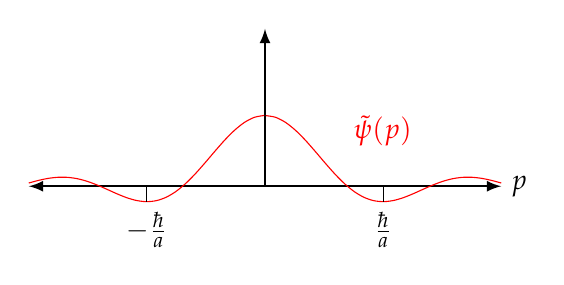
\begin{tikzpicture}
        \draw[thick, latex-latex] (-3, 0) -- (3, 0);
        \draw[thick, -latex] (0, 0) -- (0, 2);
        \node[right] at (3, 0) {$p$};
        \draw[scale=1, domain=-3:-0.01, smooth, variable=\y, red]  plot ({\y}, {(0.3*sin(deg(3*\y)))/(\y)});
        \draw[scale=1, domain=0.01:3, smooth, variable=\y, red]  plot ({\y}, {(0.3*sin(deg(3*\y)))/(\y)});
        \draw[] (-1.5, 0) -- (-1.5, -0.2);
        \node[below] at (-1.5, -0.2) {$-\frac{\hbar}{a}$};
        \draw[] (1.5, 0) -- (1.5, -0.2);
        \node[below] at (1.5, -0.2) {$\frac{\hbar}{a}$};
        \node[red, right] at (1, 0.707) {$\tilde{\psi}(p)$};
    \end{tikzpicture}};

    \node[] at (7, -0.1) {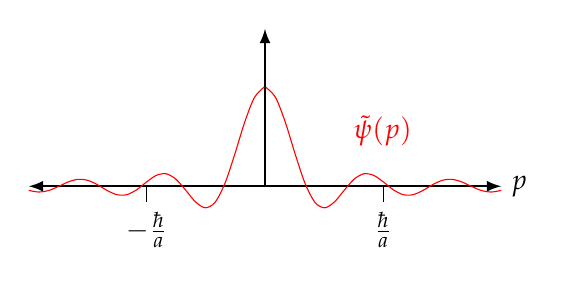
\begin{tikzpicture}
        \draw[thick, latex-latex] (-3, 0) -- (3, 0);
        \draw[thick, -latex] (0, 0) -- (0, 2);
        \node[right] at (3, 0) {$p$};
        \draw[scale=1, domain=-3:-0.01, smooth, variable=\y, red]  plot ({\y}, {0.7*0.3*(sin(deg(\y*6)))/(\y)});
        \draw[scale=1, domain=0.01:3, smooth, variable=\y, red]  plot ({\y}, {0.7*0.3*(sin(deg(\y*6)))/(\y)});
        \node[red, right] at (1, 0.707) {$\tilde{\psi}(p)$};
        \draw[] (-1.5, 0) -- (-1.5, -0.2);
        \node[below] at (-1.5, -0.2) {$-\frac{\hbar}{a}$};
        \draw[] (1.5, 0) -- (1.5, -0.2);
        \node[below] at (1.5, -0.2) {$\frac{\hbar}{a}$};
    \end{tikzpicture}};
    \draw[->] (-0.2, 3) -- (-0.2, 1.5);
    \node[right] at (-0.2, 2.25) {stretch $2\times$};

    \draw[->] (6.8, 3) -- (6.8, 1.5);
    \node[right] at (6.8, 2.25) {compress $2\times$};

    \draw[->] (2.5, 0.5) -- (4.5, 0.5);
    \node[above] at (3.5, 0.5) {FT};

    \draw[->] (2.5, 4.5) -- (4.5, 4.5);
    \node[above] at (3.5, 4.5) {FT};
\end{tikzpicture}
\end{document}